\documentclass{article}

\setlength{\parindent}{0pt}
\usepackage{cite}
\usepackage{tikz}
\newcommand\independent{\protect\mathpalette{\protect\independenT}{\perp}}
\def\independenT#1#2{\mathrel{\rlap{$#1#2$}\mkern2mu{#1#2}}}
\begin{document}
\section{Analysis}
Analysis of this project will mainly consist of comparison to th implementation fo the algorithms in R. It will compare the functionality of the algorithms on data and also the run speed of the code.\\

\subsection{Initial Skeleton Generation}
The skeleton generation code has almost identical functionality as the R implementation. Even the order in which edges are tested is the same. However the R implementation has a non-order dependent mode which is not currently implemented in the python version however could be added as an option in the future.\\

The Alarm\_1000, Asia\_1000, and Diabetes\_1000 datasets found in  all produce identical skeletons as seen in Figure \_.\\

The $\chi^2$ test for independence was not implemented in the pcalg library in R. Other independence test for discrete data, such ad the $G^2$ test, were implemented. However, the bnlearn library has an implementation of the $\chi^2$ test to use for comparison.\\

Both tests return identical results on all tested data as seen in

\subsection{PC Algorithm Edge Alignment}
\subsubsection{Asia\_10000}
	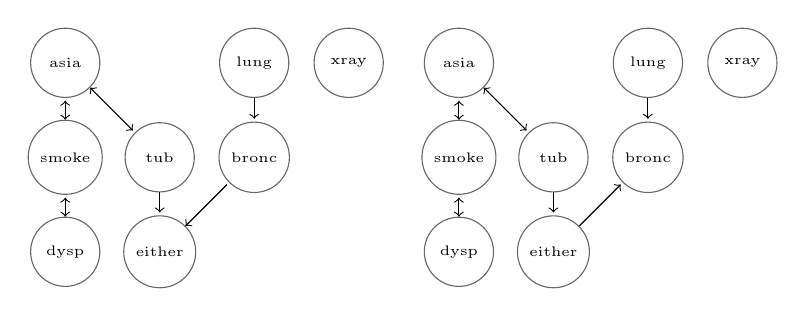
\begin{tikzpicture}[shorten >=1pt,->]
	\tikzstyle{vertex}=[circle, draw=black!60, minimum size=25pt, font=\tiny]
	\node[vertex] (asia) at (-1.2,1.2) {asia};
	\node[vertex] (tub) at (0,0) {tub};
	\node[vertex] (smoke) at (-1.2,0) {smoke};
	\node[vertex] (lung) at (1.2,1.2) {lung};
	\node[vertex] (bronc) at (1.2,0) {bronc};
	\node[vertex] (either) at (0,-1.2) {either};
	\node[vertex] (xray) at (2.4,1.2) {xray};
	\node[vertex] (dysp) at (-1.2,-1.2) {dysp};
	\draw [<->] (dysp) -- (smoke);
	\draw [<->] (smoke) -- (asia);
	\draw [<->] (asia) -- (tub);
	\draw [->] (tub) -- (either);
	\draw [<-] (either) -- (bronc);
	\draw [->] (lung) -- (bronc);[shorten >=1pt,->]
	\tikzstyle{vertex}=[circle, draw=black!60, minimum size=25pt, font=\tiny]
	\node[vertex] (asia) at (3.8,1.2) {asia};
	\node[vertex] (tub) at (5,0) {tub};
	\node[vertex] (smoke) at (3.8,0) {smoke};
	\node[vertex] (lung) at (6.2,1.2) {lung};
	\node[vertex] (bronc) at (6.2,0) {bronc};
	\node[vertex] (either) at (5,-1.2) {either};
	\node[vertex] (xray) at (7.4,1.2) {xray};
	\node[vertex] (dysp) at (3.8,-1.2) {dysp};
	\draw [<->] (dysp) -- (smoke);
	\draw [<->] (smoke) -- (asia);
	\draw [<->] (asia) -- (tub);
	\draw [->] (tub) -- (either);
	\draw [->] (either) -- (bronc);
	\draw [->] (lung) -- (bronc);
	\end{tikzpicture}


\subsubsection{Diabetes\_1000}
\subsubsection{Differences}
There are some differences in the edge orientation of the different implementations. For example, in the orient of asia\_1000 network, the edge either-bronc is oriented in opposite directions by the two implementations. This is due to the order in which the colliders were oriented in the graph. In the R implementation the triple lung, bronc, either is oriented followed by the triple tub, either bronc. This causes the edge either-bronc to be overwritten and reoriented. In the python implementation this is done in the opposite order resulting in a different network.\\

Neither order is more correct than the other however this orientation is used to estimate the final skeleton of the FCI algorithm so differences in the order can have a large knock on effect in the PAGs estimated by this algorithm.

\subsection{FCI Algorithm Final Skeleton}


\subsection{FCI Algorithm Edge Alignment}
\subsubsection{Asia\_10000}
\subsubsection{Diabetes\_1000}
\subsubsection{Differences}
\subsection{Run Speed}
\subsubsection{Method}
\subsubsection{Measurements}
\subsubsection{Algorithms}
\subsection{Skeleton Generation}
\subsubsection{Independence Tests}
The independence test was the main bottleneck of the algorithms, and was significantly slower than the R implementation. This is because the R implementation actually runs C code behind the scenes, c code is compiled rather than interpreted like python and R. This makes the code much faster.\\
 
However the independence test in the algorithm is a parameter and thus the current slow test could be replaced by a faster version which calls C code like the R implementation.\\ 
\end{document}